\documentclass[11pt, aspectratio=169]{beamer}

% --- Core Packages for Modern Documents ---
\usepackage{fontspec}      
\usepackage{unicode-math}
\usepackage{xeCJK}         
\usepackage{graphicx}      
\usepackage{minted}
\usepackage{setspace}
\usepackage{tipa}

\xeCJKsetup{CJKspace=true}

% --- Font Setup ---
\setsansfont{Noto Sans KR} %Noto Sans KR
\setmainfont{Noto Serif KR}
\setmonofont{D2Coding}

\setCJKsansfont{Noto Sans KR}  %나눔바른고딕 옛한글
\setCJKmainfont{Noto Serif KR}
\setCJKmonofont{D2Coding}

\setmathfont{Latin Modern Math}

\mode<presentation>
{
  \usetheme{default}      % or try Darmstadt, Madrid, Warsaw, Marburg...
  \usecolortheme{dove} % or try albatross, beaver, crane, dove...
  \usefonttheme{default}  % or try serif, structurebold, ...
  \setbeamertemplate{navigation symbols}{}
  \setbeamertemplate{caption}[numbered]
} 

% \setbeamertemplate{sidebar canvas right}[vertical shading][top=gray,bottom=white] 

\AtBeginSection[]{
  \begin{frame}
    \vfill % Vertically center the title
    \centering
    \begin{beamercolorbox}[sep=8pt,center,shadow=true,rounded=true]{title}
      \usebeamerfont{title}\insertsectionhead\par
    \end{beamercolorbox}
    \vfill
  \end{frame}
}

\renewcommand{\arraystretch}{1.3} % Set row height for ALL tables in the document to 1.5x

\definecolor{Highlight}{HTML}{FFF2CC} % A soft yellow

\definecolor{MonokaiBackground}{HTML}{272822}
\definecolor{blockbody}{HTML}{EEEEEE}
\setbeamercolor{block title}{bg=gray, fg=white}
\setbeamercolor{block body}{bg=blockbody, fg=black}
\setbeamertemplate{footline}{
  \hfill % Pushes the content to the right
  \usebeamercolor{page number in head/foot}
  \usebeamerfont{page number in head/foot}
  \insertframenumber{} / \inserttotalframenumber
  \hspace*{2ex} % Adds a little padding from the right edge
}

\setminted{
    style=default, % dracula, native, monokai...
    % everyminted=\color{white},
    linenos,       % Show line numbers
    % bgcolor=MonokaiBackground,
    frame=lines,   % Draw a thin frame around the code
    framesep=2mm,
    xleftmargin=6pt,
    breaklines=true
}

\title[언어의 이해]{언어의 이해}
\subtitle{강의소개}
\author{김미경}
% \institute{서울대학교}
\date{2025.9.1}


\begin{document}

\begin{frame}
  \titlepage
\end{frame}

% Uncomment these lines for an automatically generated outline.
%\begin{frame}{Outline}
%  \tableofcontents
%\end{frame}

\section{강의 계획}

\begin{frame}[t]{}

  \begin{block}{강사}
    \begin{itemize}
      \item 이름: 김미경
      \item 연락처: \underline{saltpeanuts@snu.ac.kr}
      \item 연구실: 인문대학 5동 308호 (월, 수)
    \end{itemize}
  \end{block}

  \begin{block}{수업}
    \begin{itemize}
      \item 강의 언어: 한국어
      \item 성적 부여 형태: A \textasciitilde F
      \item 성적 부여 방식: 성적평점 환산기준표(4.3만점)에 따라 부여 (\href{https://www.snu.ac.kr/academics/resources/certificate/grading}{\underline{서울대 학사행정}})
        \begin{itemize}
          \item 출석: 10점
          \item 글쓰기 과제: 1(8점), 2(14점), 3(8점)
          \item 중간고사: 30점
          \item 기말고사: 30점
        \end{itemize}
    \end{itemize}    
  \end{block}
\end{frame}

\begin{frame}[t]{}
  \begin{block}{수업목표}
    \setstretch{1.6}이 수업에서는 \textbf{인간 언어의 특성과 구조}에 대해 살펴보고 \textbf{언어학의 다양한 분야}를 소개한다. \underline{언어의 소리, 형태, 구조, 의미} 등을 과학적으로 분석함으로써 자신이 사용하는 언어를 메타적으로 바라보는 시각을 키운다. 언어 \underline{변화}와 \underline{변이}의 양상 및 언어의 \underline{여러 유형}을 살피고, 언어가 \underline{문자}로 기록되는 방식을 살펴 언어의 역동성과 다양성을 접하도록 한다.
  \end{block}
  \begin{block}{추가로...}
    \begin{itemize}
      \item 연구 대상으로서의 언어 개관
      \item 사람이 언어를 처리하는 방식
      \item 서로 다른 언어가 접촉하는 양상
    \end{itemize}
  \end{block}
\end{frame}

\begin{frame}[t]{}
  \begin{block}{교재}
    Language files : materials for an introduction to language and linguistics
    \begin{itemize}
      \item \href{https://ohiostatepress.org/books/titles/9780814258354.html}{\underline{출판사 공식 페이지}}
      \item \href{https://snu-primo.hosted.exlibrisgroup.com/permalink/f/1l6eo7m/82SNU_INST21929717540002591}{\underline{중앙도서관 페이지}} (참고자료실\_강의도서)
    \end{itemize}
  \end{block}      
  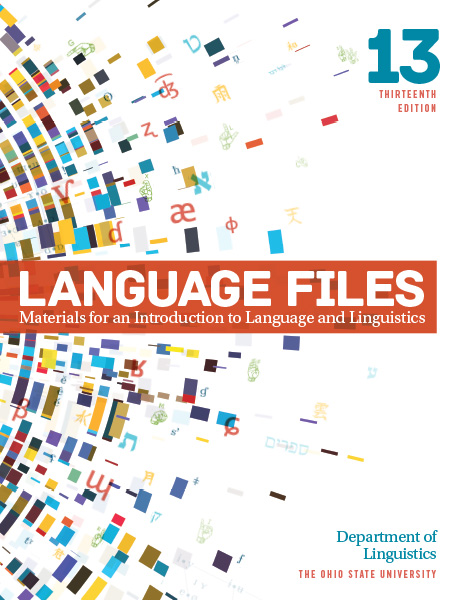
\includegraphics[height=0.6\textwidth]{img/9780814258354.jpg}
\end{frame}

\begin{frame}[t]{}
  \begin{block}{주차별 수업 내용: eTL 모듈 참조}
    \begin{itemize}
      \item 월: 지난 주제 강의에 대한 퀴즈 및 해설
      \item 수: 새 주제 강의
    \end{itemize}     
  \end{block}

  \begin{block}{공휴일 정책: 수업 없음. 자율학습일.}
    \begin{itemize}
      \item 추석(10월 6일, 10월 8일)
      \item 개교기념일(10월 15일)
    \end{itemize}      
  \end{block}
  \begin{block}{출석 (전자출결)}
    결석 사유가 생기면 mySNU “출석인정신청” 메뉴 이용
    \begin{itemize}
      \item mySNU - 학사행정 - 수업/성적 - 수업 - 출석인정신청
    \end{itemize}
  \end{block}

\end{frame}

\begin{frame}[t]{}
    \begin{block}{시험 일정}
      \begin{itemize}
        \item 중간고사: 10월 20일
        \item 기말고사: 12월 10일
      \end{itemize}       
    \end{block}

  \begin{block}{중간/기말고사 평가 기준 (문제당 3점 만점)}
    \begin{itemize}
      \item 내용의 정확성 (필수 정보 모두 포함, 오류 없음): 2.5점
      \item 이해의 탁월성 (개념과 용어를 깊이 있게 설명): +0.5점
      \item 정보 누락 또는 내용 오류: 항목당 -0.5점
    \end{itemize}
  \end{block}

\end{frame}

\begin{frame}[t]{}

    \begin{block}{글쓰기 과제 일정}
        \begin{itemize}
          \item 과제 1: 9월 8일 \textasciitilde 9월 29일
          \item 과제 2: 10월 13일 \textasciitilde 11월 3일
          \item 과제 3: 11월 24일 \textasciitilde 12월 8일
        \end{itemize}      
    \end{block}  

  \begin{block}{과제 평가 기준 (1점 단위 감점)}
    \begin{itemize}
      \item 글의 완성도 (각 문단이 논리적으로 연결되고 통일성을 이룸)
      \item 수업에서 다룬 핵심 개념과 용어를 정확하게 사용
      \item 내용의 평이함 (쉬운 문장과 적절한 예시 사용)
      \item 분량 준수 
    \end{itemize}
  \end{block}

\end{frame}

\section{강의 주제 소개}

\begin{frame}[t]{}
  \begin{block}{이 발음과 저 발음은 왜 다르게 들리지?}
    \href{https://youtube.com/watch?v=dVKh6fSxbkE}{\underline{https://youtube.com/watch?v=dVKh6fSxbkE}}
  \end{block}
  광고 첫부분의 ‘The 매일 두유 is clean...’의 ‘매일 두유’와, 본인이 발음하는 ‘매일 두유’를 비교해 보세요. 동일한가요?
\end{frame}

\begin{frame}[t]{}
  \begin{block}{단어를 왜 이렇게 쪼개지?}
    \begin{center}
      \setstretch{1.6}pneumonoconiosis\\
      pneumonoultramicroscopicsilicovolcanoconiosis\\
      \textipa{("nju:m@nou""2ltr@""maikr@""skApIk"sIlI""kouvAl""keinou""kouni"ousIs)}\\
      {\small pneu‧mo‧no‧ul‧tra‧mi‧cro‧sco‧pic‧si‧li‧co‧vol‧ca‧no‧co‧ni‧o‧sis}\\
      pneumono-ultramicroscopic-silico-volcano-coniosis\\
      pneumon-o-, ultra-micro-scop-ic, silico-, volcano, coni-osis\\
      {\small 주로 화산에서 발견되는 아주 미세한 규소 먼지를 흡입하여 허파에 쌓여 생기는 만성 폐질환}      
    \end{center}
  \end{block}  
\end{frame}

\begin{frame}[t]{}
  \begin{block}{문장 늘리기 게임, 어디까지?}
    \begin{center}
      \setstretch{1.6}태희가 \,\,\,\, 늦었다 \\
      태희가 수업에 늦었다 \\
      태희가 어제 버스를 놓쳐서 수업에 늦었다 \\
      태희가 어제 늦잠을 자서 버스를 놓쳐서 수업에 늦었다 \\
      ...
    \end{center}
  \end{block}
  우리는 어디까지 이 문장을 늘릴 수 있을까요?
\end{frame}

\begin{frame}[t]{}
  \begin{block}{어, 말이 안 통했는데?}
    A: 고향이 어디야? \\
    B: 용인입니다.\\
    A: 옛날 사람들은 ‘아~ 자연농원 있는 데?’\\
    (다함께 웃음)\\
    B: 나름 그냥 도시였어요!\\
    A: 아 그게 아니라, 에버랜드 있잖아?\\
    B: 네\\
    A: 거기가 옛날 이름이 자연농원 맞지?\\
    C: 어어\\
    B: 아\dots\\
    A: 그래서 웃은 거야\\
    B: 난 또 그냥 촌이라고~\\
    C: 에이, 용인을 무시한 게 아니야~ 
  \end{block}
  A와 B는 왜 말이 통하지 않았을까요?
\end{frame}

\begin{frame}[t]{}
  \begin{block}{그런 말은 꺼내지도 않았는데...?}
    A: 군대는 갖다 오셨어요?\\
    B: 예! 갖다 왔어요.\\
    A: 어디 근무하셨어요?\\
    B: 전 해병대 다녀왔어요.\\
    A: 어~ 그러셨구나. 몇 기\dots\\
    B: (점점 목소리가 작아짐) 천 백\dots 육십\dots 칠기\dots 해병대 나오셨어요?\\
    A: (웃음) 이러면은, 다 쫄더라구요\\
    (다함께 웃음)\\
    A: 아이 이렇게 기수를 물어보면, 보통 해병대 나오신 분들은, 되게 긴장을 하시더라고요. 에이 저는 그냥 육군 나왔어요.
  \end{block}
  B는 ‘몇 기’라는 질문에 왜 긴장했을까요?
\end{frame}

\begin{frame}[t]{}
  \begin{block}{중국 사람들은 어순이 똑같으니 영어 배우기 쉽지 않아?}
    \begin{tabular}{llll}
      \textbf{중국어} & \textbf{영어} & \textbf{한국어} & \textbf{일본어} \\
      wǒ (나는) & I & 나는 & watashi wa(나는) \\
      xǐhuān (좋아한다) & like & 커피를 & kōhī ga(커피가) \\
      kāfēi (커피) & coffee & 좋아한다 & suki da (좋다) \\
    \end{tabular}
  \end{block}
  중국어는 영어와 비슷한가요? 한국어는 일본어와 비슷한가요?
\end{frame}

\begin{frame}[t]{}
  \begin{block}{언어가 쪼개진다고?}
    \begin{center}
      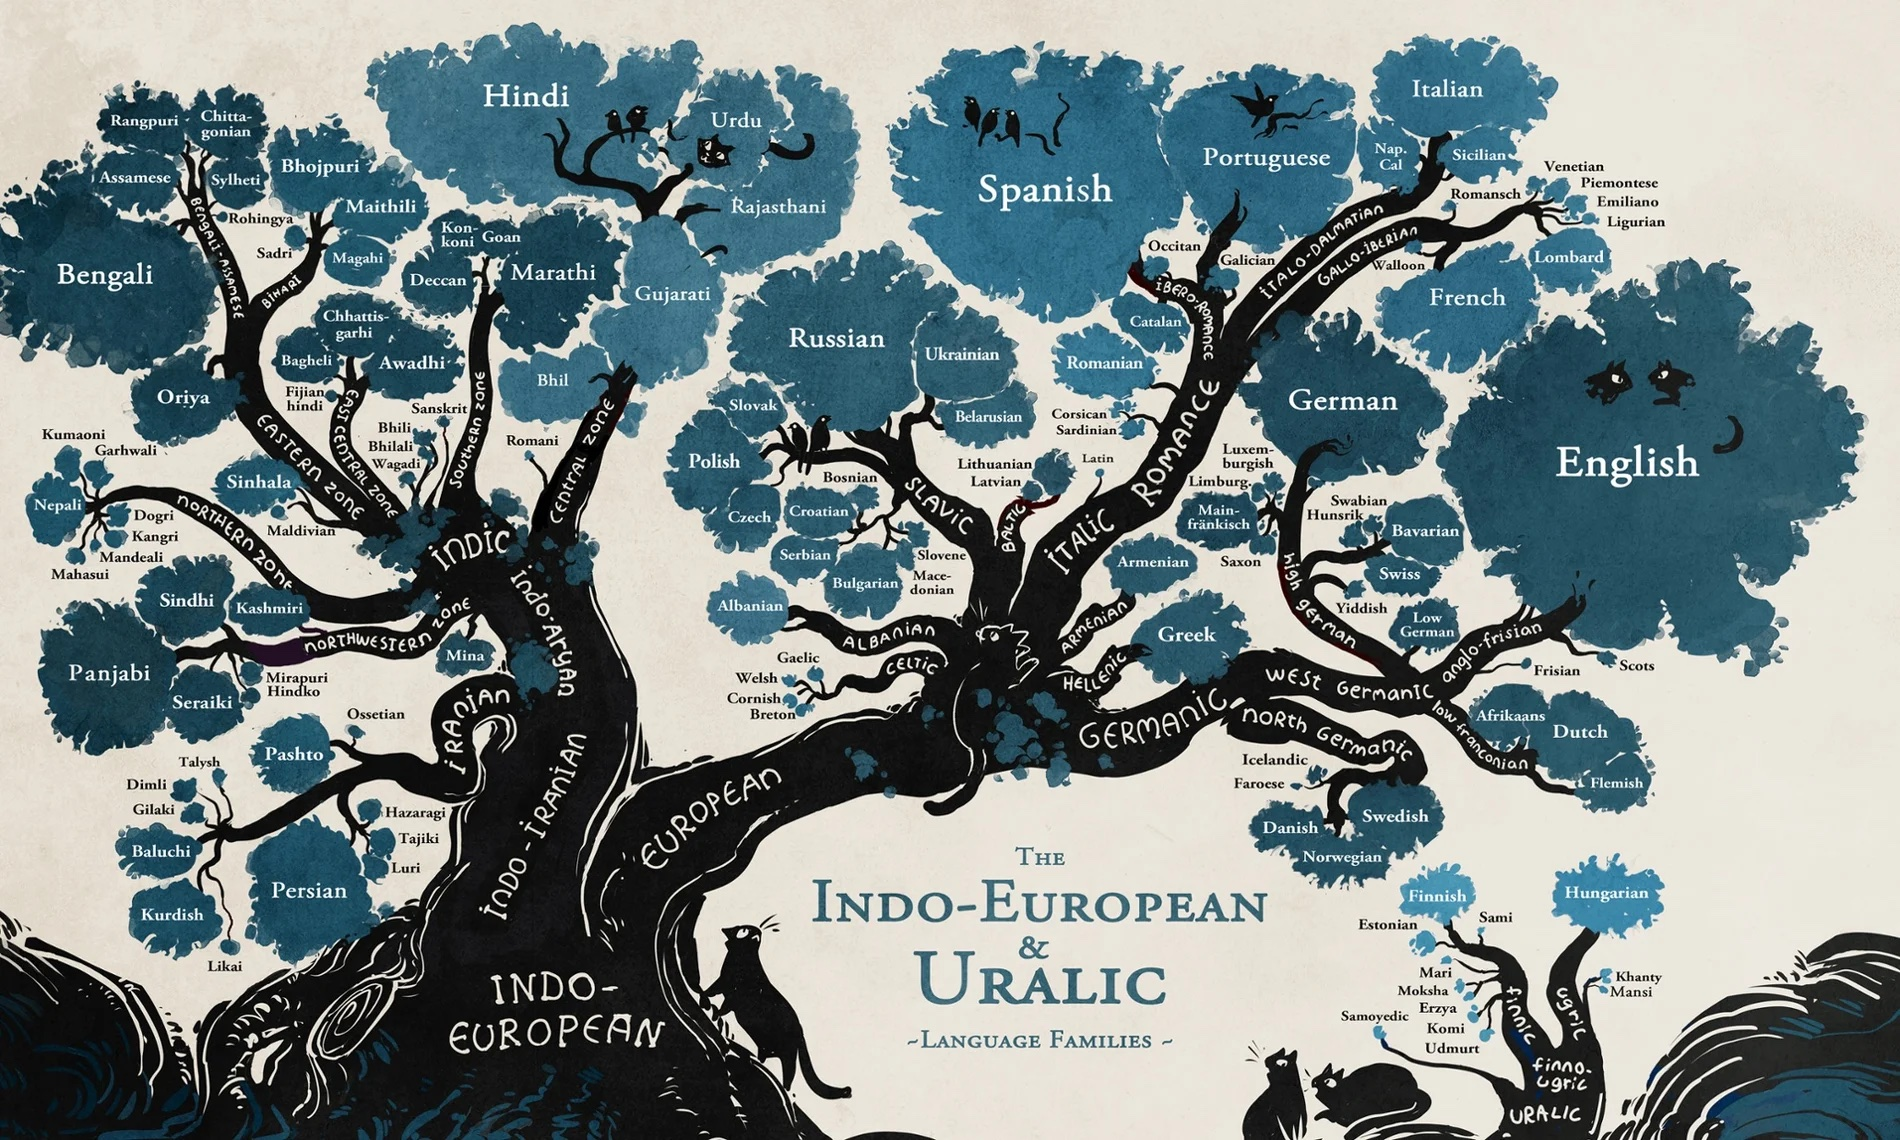
\includegraphics[width=0.8\textwidth]{img/fe0733eb-8981-441d-9323-a9c635347ab8-2060x1236.jpg}\\
      \href{https://www.theguardian.com/education/gallery/2015/jan/23/a-language-family-tree-in-pictures}{The Guardian ‘A language family tree - in pictures’ 2015. 1. 23}
    \end{center}
  \end{block}
\end{frame}

\begin{frame}[t]{}
  \begin{block}{우리가 어떻게 말을 하는 거지?}
    \begin{itemize}
      \item 문제 유형 1 \\ \href{https://youtube.com/watch?v=JWC-cVQmEmY}{https://youtube.com/watch?v=JWC-cVQmEmY}
      \item 문제 유형 2 \\ \href{https://youtube.com/watch?v=3oef68YabD0}{https://youtube.com/watch?v=3oef68YabD0}
    \end{itemize}
  \end{block}
  두 영상에 등장한 사람들은 왜 보통 사람들처럼 말하지 못할까요?
  \vfill
  \begin{block}{우리가 어떻게 말을 배우는 거지?}
    \href{https://youtu.be/RE4ce4mexrU}{https://youtu.be/RE4ce4mexrU}
  \end{block}
  어린이는 어떻게 말을 배울까요?
\end{frame}

\begin{frame}[t]{}
  \begin{block}{왜 같은 한국어인데 다르다고 하지?}
    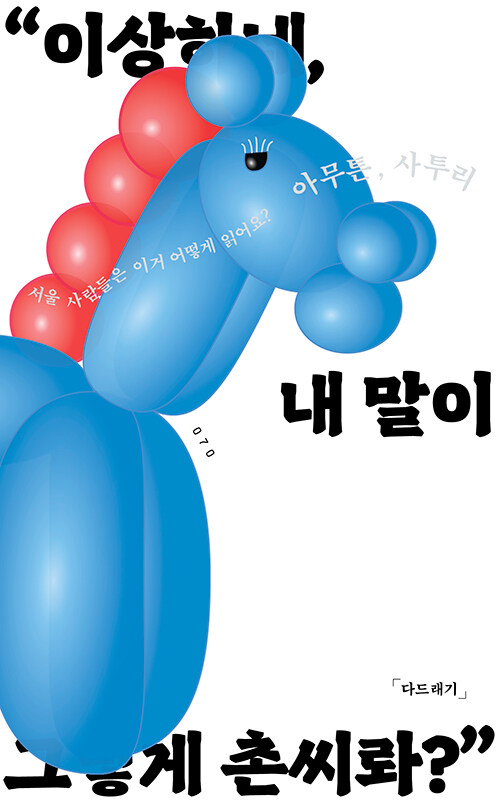
\includegraphics[width=0.5\textwidth]{img/K812933112_f.jpg}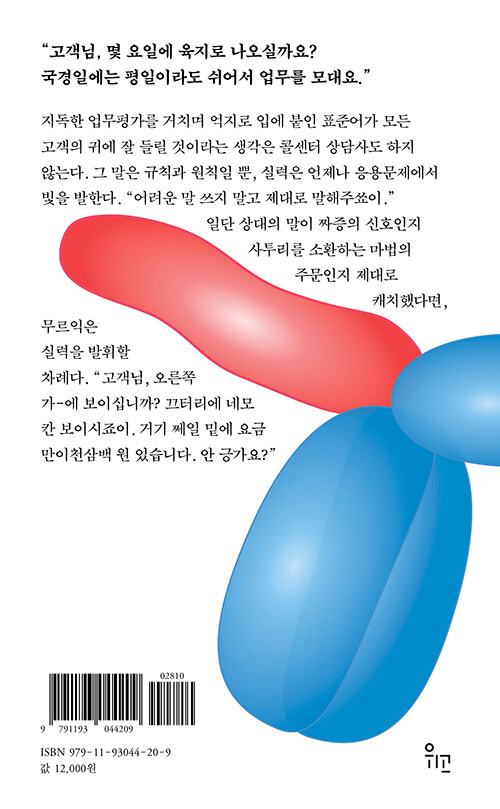
\includegraphics[width=0.5\textwidth]{img/K812933112_b.jpg}    
  \end{block}
\end{frame}

\begin{frame}[t]{}
  \begin{block}{여러 언어가 함께 쓰인다는 건 어떤 걸까?}
    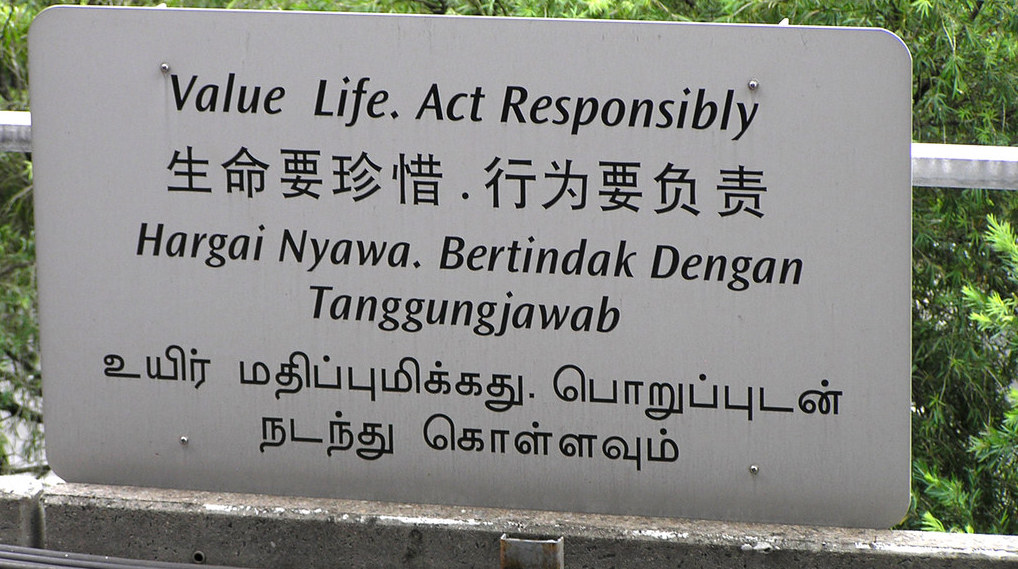
\includegraphics[width=1.0\textwidth]{img/550304175_fbcaca2d23_b.jpg}
  \end{block}
\end{frame}

\section{강의하지 않는 주제}

\begin{frame}[t]{}
  \begin{block}{언어학은 무엇을 하지 않는가}
    \begin{itemize}
      \item 토익 만점 일주일 완성
      \item n개 국어 유창하게 하기
      \item 맞춤법 지켜쓰기
      \item 바르고 고운말 하기
      \item 글쓰기 잘 하는 법
      \item 타인을 설득하는 화술
      \item 수학의 언어
      \item 음악의 언어
      \item 동물의 언어
      \item 컴퓨터 프로그래밍 언어
    \end{itemize}
  \end{block}
\end{frame}

\begin{frame}[t]{}
  \begin{block}{언어학은 무엇을 하지 않는가}
    \begin{itemize}
      \item 언어의 기원
       \begin{itemize}
        \item 버전 1: 가장 오래된 언어는 무엇인가? 
        \item 버전 1의 변형: 언어의 역사를 거슬러 올라가면 가장 최초의 형태는 어떤 모습이었을까? 
        \item 버전 2: 영장류는 말을 할 수 없는데 인간은 말을 할 수 있다, 어떻게? 
       \end{itemize}
    \end{itemize}
    \begin{center}
      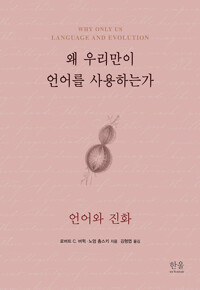
\includegraphics[width=0.2\textwidth]{img/8946065338_1.jpg} 
      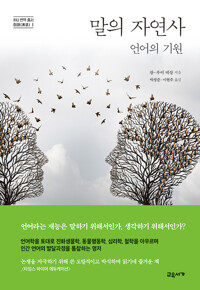
\includegraphics[width=0.2\textwidth]{img/k962831307_1.jpg} 
      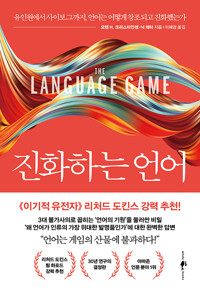
\includegraphics[width=0.2\textwidth]{img/k432832329_2.jpg} 
      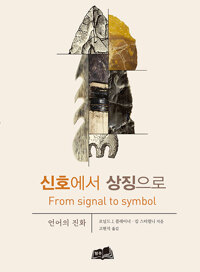
\includegraphics[width=0.2\textwidth]{img/k172938313_1.jpg}
    \end{center}
  \end{block}
\end{frame}

\end{document}